\documentclass[
    12pt,
    bibliography=totoc,
    listof=totoc
]{scrartcl}

\RequirePackage{amsmath}            % Math
\RequirePackage{amsfonts}
\RequirePackage{amssymb}
\RequirePackage{graphicx}           % Include graphics to document
\RequirePackage[ngerman]{babel}     % New german spell checking
\RequirePackage[T1]{fontenc}        % Font
\RequirePackage[hyphens]{url}       % Line break support in URL
\RequirePackage[absolute]{textpos}  % place at absolute coordinates on title page
\RequirePackage[utf8]{inputenc}         % Universal encoding
\RequirePackage{helvet}
\RequirePackage{setspace}
\RequirePackage[numbers]{natbib}
\RequirePackage{fancyhdr}

\usepackage[paper=a4paper, top=40mm, bottom=20mm, left=40mm, right=20mm]{geometry}

\title{Chat Client}
\subtitle{Entwicklung eines p2p Chat Clients auf Basis von klassischen Client-Server Protokollen}
\author{Rebeka Fischer \\}
\date{06.02.2024}

\pagestyle{fancy}
\chead{\thepage}
\cfoot{}
\lhead{}
\rhead{}
\begin{document}
\onehalfspace
\makeatletter
%\maketitle{}
\thispagestyle{empty}
\begin{titlepage}{

    \begin{center}
        \includegraphics[width=2.3cm]{Images/fomLogo.pdf}

        \vspace{10mm}
        \fontsize{20pt}{20pt}\selectfont
        \textbf{FOM Hochschule für Ökonomie \& Management}\\
    \end{center}


    % \begin{textblock*}{\paperwidth}{57mm, 72mm}
    %     \begin{center}
    %         \vspace{2mm}
    %         Berufsbegleitender Studiengang in Wirtschaftsinformatik
    %         \\
    %         3.Semester
    %     \end{center}
    % \end{textblock*}   
        
    %\begin{textblock*}{\paperwidth} (0mm, 98mm)  % x has offset of 2 mm
        %\begin{minipage}[t][0cm][b]{\textwidth}
        % kind of doc here
        %\fontsize{10pt}{10pt}
        %\fontfamily{opensans}
        %\selectfont
        \begin{center}
            % author of doc
            \normalsize{Berufsbegleitender Studiengang in Wirtschaftsinformatik} \\
            3.Semester \\
            \vspace{10mm}
            \large{\textbf{Seminararbeit}}\\
            in IT Infrastruktur \\
            \vspace{15mm}
            \fontsize{20pt}{20pt}\selectfont
            \textbf{\@title} \\
            \vspace{2mm}
            \fontsize{15pt}{15pt}\selectfont
            \@subtitle \\
            \vspace{15mm}
            \fontsize{15pt}{15pt}\selectfont
            \@author
            \vspace{30mm}
        \end{center}
        % \begin{flushleft}
        %     Dozent: Christian Frank \\
        %     \vspace{5mm}
        %     Matrikelnummer: 674516\\
        %     \vspace{5mm}
        %     Abgabedatum: 24.02.2024\\
        % \end{flushleft}
        %\end{minipage}
    %\end{textblock*}




    %\begin{minipage}[b][14.5cm][b]{\textwidth}
        
        \begin{flushleft}
            \fontsize{12pt}{12pt}
            \fontfamily{opensans}
            \selectfont
            Dozent: Christian Frank \\
             \vspace{5mm}
             Matrikelnummer: 674516\\
             \vspace{5mm}
             Abgabedatum: 24.02.2024\\
        \end{flushleft}
    %\end{minipage}
 
}\end{titlepage}

\newpage
\pagenumbering{Roman}
\setcounter{page}{2}
\tableofcontents
\newpage
\listoffigures
\newpage
\pagenumbering{arabic}
\setcounter{page}{1}
\section{Einleitung}
Im Rahmen dieser Arbeit soll ein peer to peer Chat client entwickelt werden, der die Kommunikation in einer Gruppe im lokalen Netzwerk ermöglicht. 
Die Arbeit richtete sich an ein fachkundiges Publikum und setzt beim Leser ein grundlegendes Verständnis für Computernetzwerke voraus. 
Das Hauptziel besteht darin, einen funktionierenden Chatroom mit direkter Nachrichtenübertragung zu bauen.
Es handelt sich hierbei um einen einzigen Chatroom für alle Teilnehmer, private Chats zwischen einzelnen Nutzern sind nicht möglich. 
Die Chat Anwendung beschränkt sich auf das Versenden und Empfangen von Nachrichten, Funktionen wie das Versenden von Audionachrichten oder Bilder sind nicht Bestandteil. 
Das Verschicken und Zustellen von Nachrichten, sowie das Auffinden, Beitreten und Verlassen des Chats sollen ohne zusätzliche Infrastrukturkomponenten, wie ein externer Server, möglich sein.
Die Nachrichten werden direkt an die Geräte der anderen Teilnehemr im Netzwerk geschickt. 
Angesichts der weit verbreiteten Verfügbarkeit von qualitativ hochwertigen Frameworks für client-server Applikationen und der vergleichsweise geringen Anzahl an peer-to-peer Frameworks mit ähnlicher Güte stellt sich die Frage: 
Ist es möglich mit Client-Server-Technologien einen peer to peer Chat Client zu entwickeln?
\section{Grundlagen}
Für die Entwicklung einer Chat-Anwendung gibt es verschiedene Möglichkeiten zur technischen Umsetzung.
Häufig wird die Client-Server Architektur verwendet. Diese ist das am häufigsten genutze Architekturmodell. 
Der Computer nimmt die Rolle des Clients ein und fragt beim Server Daten an. 
Der Server ist normalerweise ein leistungsstarker Computer, der Daten speichert und sie auf Anfrage zurück gibt.
Client und Server sind über das Netzwerk miteinander verbunden. 
Bei einem Chat client finden zwei Prozesse für die Kommunikation statt.
Zuerst sendet der Client eine Nachricht über das Netzwerk an den Server und wartet auf eine Antwortnachricht. 
Wenn der Server den request des Clients erhält, gibt er eine Antwort mit den geforderten Daten zurück. 
\cite{tanenbaum96}
\\
\\
Dem Client-Server-Modell entgegen steht das Peer-To-Peer-Modell.
Einzelne Computer treten direkt über das Netzwerk miteinander in Kontakt und können kommunizieren.
Es werden Pakete an User geschickt, die als Teil der vorgesehenen Gruppe identifiziert wurden. 
Somit ist jeder Computer ein peer, er kann als Client gegenüber anderen Geräten agieren, aber auch als Server.
Durch das Einnehmen der Client- und Serverfunktion eines jeden Computers ist kein seperater Server notwendig.
Es werden nur die einzelnen Endgeräte benötigt und eine Netzwerkverbindung.
\cite{tanenbaum96}
%was für übertragungsmodi, was unterschied p2p client server, wie machen kann, wie man was baut, an frage annähern  
\section{Umsetzung}
%was für komponenten braucht, etwas was auffinden ermöglicht, etwas was als server fungiert, jeder client ist server und client, wie finde ich server
%Erst erklären was ich machen: wie hab ich es gemacht. Hier auch diagramme einfügen 
\subsection{Idee}
%Um einen funktionierenden Chatroom zu bauen, werden verschiedene Komponenten für unterschiedliche Aufgaben benötigt. 
Die Applikation soll es ermöglichen, dass mehrere Nutzer im selben Netzwerk miteinander chatten können. 
Dafür müssen zu Beginn andere Teilnehmer im Netzwerk gefunden werden.
Da kein Server angefragt werden kann, um herauszufinden welche Teilnehmer es gibt, müssen sich die Geräte untereinander finden. Mithilfe eines Multicast könnte der neue User 
herausfinden, wer bereits alles im Chatroom und im Netzwerk vorhanden ist. 
Wurde ein Chatteilnehmer gefunden, muss sowohl die Adresse als auch der Name des jeweils anderen herausgefunden und gespeichert werden. 
Somit weiß jeder User welche anderen Teilnehmer vorhanden sind. 
Nach dem Beitritt können Nachrichten verschickt werden. Jeder User kann alle gesendeten Nachrichten lesen, da die Nachricht an jede vorhandene Adresse der einzelnen Teilnehmer verschickt wird.
Möchte ein User den Chatroom verlassen muss sichergestellt werden, dass dieser User nach dem Austritt keine weiteren Nachrichten erhält. 
Mit dem Verlassen des Chatrooms müssen die anderen Geräte informiert werden, dass diese Adresse nicht mehr vorhanden ist und keine Nachrichten dahingeschickt werden.
\\
\subsection{Ablauf}
Beim Starten der Chat-Anwendung findet eine Initialisierung statt. 
Der Client soll mithilfe eines mdns Broadcast andere Chatteilnehmer finden.
Wurde ein anderer Teilnehmer gefunden bekommt der Client eine mdns Antwort mit der IP Adresse des Teilnehmers.
Die IP Adresse wird von dem DiscoveryService in eine Userliste eingetragen. 
An jede gefundene IP Adresse wird eine Startmessage mit eigener IP Adresse und Name über HTTP geschickt. Der andere Teilnehmer kann somit den neuen 
User in seiner Liste ergänzen und ebenfalls eine Startmessage mit seinem Namen als Antwort schicken. Der neue Client ergänzt in seiner Userliste 
den Namen. Damit ist die Initialisierung abgeschlossen. 
\begin{figure}[ht]
    \centering
    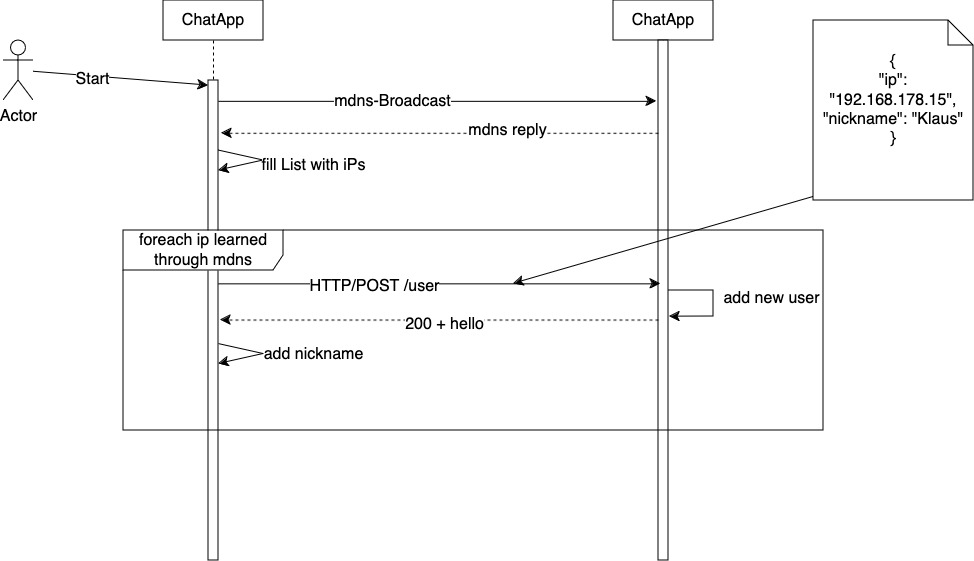
\includegraphics[scale=0.4]{Images/Initialisierung_Sequenzdiagramm.jpg}
    \captionbelow{Initialisierung}
\end{figure}
\\
\\
Nachdem man dem Chatroom beigetreten ist können Nachrichten verschickt werden. Der User schreibt eine Nachricht. 
Um diese Nachricht zu verschicken muss der Client in der Userliste alle IP Adressen der Teilnehmer nachschauen. Die Nachricht wird anschließend 
an jede einzelne IP Adresse geschickt. Das Versenden der Nachrichten findet ebenfalls mittels HTTP statt.
\begin{figure}[h]
    \centering
    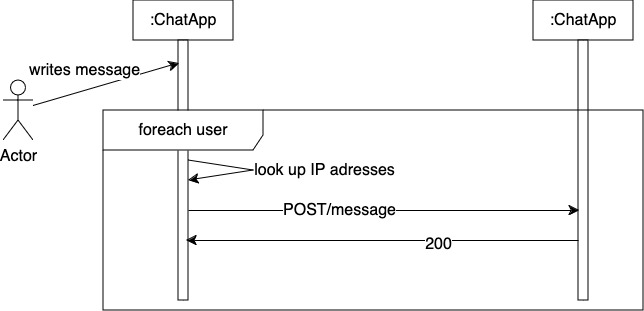
\includegraphics[scale=0.4]{Images/Conversation_Sequenzdiagramm.jpg}
    \captionbelow{Kommunikation}
\end{figure}
\\
Um den Chatroom zu verlassen wird wieder über HTTP eine Exitmessage an alle Teilnehmer gesendet. Die Exitmessage enthält wie die Startmessage den eigenen Namen und IP Adresse.
Der User wird von den anderen Teilnehmern aus der Userliste entfernt und der Client ist somit dem Chatroom ausgetreten. 
\begin{figure}[h]
    \centering
    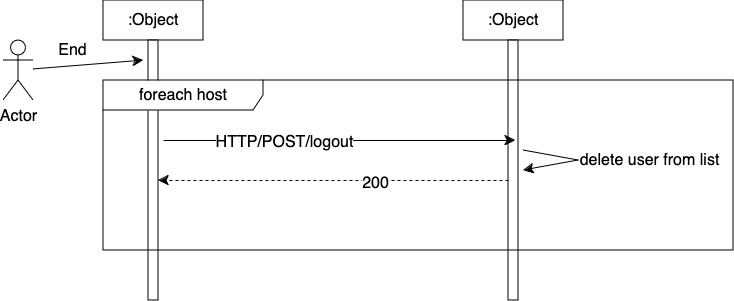
\includegraphics[scale=0.4]{Images/Exit_Sequenzdiagramm.jpg}
    \captionbelow{Exit}
\end{figure}
\\

\subsection{Aufbau und Komponenten}
Der Chat client setzt sich im wesentlichen zusammen aus:
\begin{itemize}
    \item DiscoveryService
    \item Transmitter
    \item Receiver
    \item ConfigData
    \item Message types
\end{itemize} 
Um mit dem chatten starten zu können wird der DiscoveryService benötigt. 
Er ist für den Multicast und das Eintragen der Teilnehmer in die Userliste verantwortlich,
Der Receiver ist für das Empfangen der Startmessage, der normalen Nachrichten und der Exitmessage zuständig.
Der Transmitter übernimmt die Funktion des Sendens der Nachrichten. 
In der ConfigData ist die Userliste angelegt, mit allen eingetragenen Teilnehmern des Cahtrooms und die eigenen Daten.
Die Message types definieren die einzelnen Typen und den Aufbau der unterschiedlichen Messagearten. Diese unterteilen sich in StartMessage, Message und ExitMessage.

\subsection{Funktionalität}
%Wird die Anwendung gestartet beginnt der DiscoveryService mit einem Multicast nach anderen Teilnehmern zu suchen. Hierfür wurde die zeroconf library verwendet.
%....
%Die gefundenen Teilnehmer werden mit ... in die angelegte UserLsite der ConfigData eingetrage....
%Die ConfigData besteht aus dem eigenem Namen, der eigenen IP Adresse, die mithilfe der Klasse IPv4Adress herausgesucht wird und der Portnummer.
%Des Weiteren ist in der ConfigData die Userliste angelegt. Die User sind in einem Dictonary angelegt, wobei jeder IP Adresse der passende Name zugeordnet wird.









\section{Ergebnisse}
Alle Anforderugen wurden erfolgreich umgesetzt. 
Somit ist es möglich eine peer to peer Chat-Anwendung zu bauen mit client-server Technologie.
Mit dem Programmstart gibt der User seinen Nutzernamen ein und die API wird gestartet. 
Das Programm sucht automatisch nach anderen Nutzern im Netzwerk, ohne einen externen Server anfragen zu müssen.
Es können problemlos Nachrichten an die verschiedenen Teilnehmer geschickt werden, da durch die Speicherung der vorhandenen User die Nachrichten an jeden User direkt verschickt werden.
Dadurch entsteht problemlos ein Chatroom, in dem jeder Benutzer Nachrichten empfangen und verschicken kann. 
Angezeigt wird sowohl der Name der Person, die die Nachricht verschickt hat, als auch dahinter die Nachricht selbst. 

\section{Fazit}
Im Rahmen dieser Arbeit wurde ein peer-to-peer Chat client mit client-server Technologie erstellt. 
Nach der theoretischen Ausarbeitung der Funktionsweise der Chatapplikation wurde eine konkrete Umsetzung in Python geschrieben um zu testen,
ob eine praktische Anwendung möglich ist.
Das Programm stellt die Grundfunktionen einer Chatapplikation dar, kann jedoch noch erweitert werden. 
Momentan liegt der Fokus auf dem Austausch von Nachrichten, es könnte ergänzt werden durch Funktionen wie Bilder oder Emojis versenden. Zudem werden
die Nachrichten nicht gespeichert, mit Verlassen des Chats wird auch der Chatverlauf gelöscht und kann nicht bei erneutem Beitritt wiederhergestellt werden.
Des Weiteren könnte man den Exitprozess verbessern. Die Dauer des Austretens aus dem Chatroom erhöht sich, je mehr Teilnehmer vorhanden sind.
Der Ablauf könnte verbessert werden, damit bei einer hohen Tielnhemerzahl das Verlassen und Abmelden schneller ausgeführt wird.
\\
Für eine temporäre Kommunikation innerhalb des selben Netzwerks ist die peer-to-peer Methode für einen Chatroom geeignet, allerdings ist von einem 
öffentlichen Gebrauch abzuraten. Je größer die Teilnehmermenge des Chatrooms wird, desto unübersichtlicher wird der Chatverlauf und es besteht derzeit keine 
Funktion private Chats zu öffnen, sowie einen Verlauf zu speichern.
Zusätzlich dürfte kaum Bedarf in Firmen oder im privaten Leben bestehen, einen einzigen großen Chatroom zu haben, der nur den reinen Nachrichtenaustausch ermöglicht.
Dennoch eignet sich die Anwendung für eine kleine Gruppe, wie beispielsweise Studenten in einer Bibliothek oder einem Hörsaal, um sich schnell über ein Thema auszutauschen.
\newpage

\bibliographystyle{IEEEtranN}
\bibliography{literatur/literatur}
\end{document}